\documentclass[10pt]{article}

% ---------------------------------------------------------------------------
% NeurIPS page layout (reproduces the geometry, fonts and title block of the
% official neurips_20xx.sty). To use the official file instead, delete this
% block and add \usepackage[preprint]{neurips_2025} (or the current year).
% ---------------------------------------------------------------------------
\makeatletter
\setlength{\paperheight}{11in}
\setlength{\paperwidth}{8.5in}
\setlength{\oddsidemargin}{0.5in}
\setlength{\evensidemargin}{0.5in}
\setlength{\marginparwidth}{0.07in}
\setlength{\topmargin}{-0.625in}
\setlength{\headheight}{12pt}
\setlength{\headsep}{25pt}
\setlength{\textheight}{9in}
\setlength{\textwidth}{5.5in}
\setlength{\footskip}{30pt}
\setlength{\parindent}{0pt}
\setlength{\parskip}{5.5pt}
\renewcommand{\normalsize}{\@setfontsize\normalsize\@xpt\@xipt
  \abovedisplayskip 7pt plus 2pt minus 5pt
  \belowdisplayskip \abovedisplayskip
  \abovedisplayshortskip 0pt plus 3pt
  \belowdisplayshortskip 4pt plus 3pt minus 3pt}
\normalsize
\renewcommand{\section}{\@startsection{section}{1}{\z@}
  {-2.0ex \@plus -0.5ex \@minus -0.2ex}{1.5ex \@plus 0.3ex \@minus 0.2ex}
  {\large\bf\raggedright}}
\renewcommand{\subsection}{\@startsection{subsection}{2}{\z@}
  {-1.8ex \@plus -0.5ex \@minus -0.2ex}{0.8ex \@plus 0.2ex}
  {\normalsize\bf\raggedright}}
\renewcommand{\paragraph}{\@startsection{paragraph}{4}{\z@}
  {1.5ex \@plus 0.5ex \@minus 0.2ex}{-1em}{\normalsize\bf}}
\def\toptitlebar{\hrule height 4pt \vskip 0.25in \vskip -\parskip}
\def\bottomtitlebar{\vskip 0.29in \vskip -\parskip \hrule height 1pt \vskip 0.09in}
\renewcommand{\maketitle}{%
  \par\begingroup
  \thispagestyle{plain}
  \vbox{\hsize\textwidth \linewidth\hsize
    \vskip 0.1in
    \toptitlebar
    \centering{\LARGE\bf \@title\par}
    \bottomtitlebar
    \def\And{\end{tabular}\hfil\linebreak[0]\hfil
      \begin{tabular}[t]{c}\bf\rule{\z@}{24pt}\ignorespaces}
    \begin{tabular}[t]{c}\bf\rule{\z@}{24pt}\@author\end{tabular}
    \vskip 0.3in \@minus 0.1in}
  \endgroup}
\renewenvironment{abstract}{%
  \vskip 0.075in
  \centerline{\large\bf Abstract}
  \vspace{0.5ex}
  \begin{quote}}{\par\end{quote}\vskip 1ex}
\makeatother
% ---------------------------------------------------------------------------

\usepackage[utf8]{inputenc}
\usepackage[T1]{fontenc}
\usepackage{times}
\usepackage[numbers,sort&compress]{natbib}
\usepackage{amsmath,amssymb,amsthm}
\usepackage{booktabs}
\usepackage{graphicx}
\usepackage{microtype}
\usepackage{nicefrac}
\usepackage{xcolor}
\usepackage[hidelinks]{hyperref}
\usepackage{url}

\newtheorem{proposition}{Proposition}
\newtheorem{lemma}{Lemma}
\newcommand{\1}{\mathbf{1}}
\newcommand{\E}{\mathbb{E}}
\newcommand{\RPS}{\mathrm{RPS}}

\title{Forecasting First-Innings Totals in Men's T20 Internationals\\with a Proper Scoring Rule}

\author{%
  Abhishek Shukla\\
  University of California, Berkeley\\
  \texttt{abhishek.shukla@berkeley.edu}
}

\setlength{\emergencystretch}{2em}
\begin{document}
\maketitle

\begin{abstract}
We study probabilistic forecasting of the final first-innings total in men's Twenty20 International (T20I) cricket, issued before the first ball and after overs 6, 10 and 15. Ball-by-ball records from Cricsheet let us replay every historical innings and build features using only information available at the moment of the forecast. We score full predictive distributions with the Ranked Probability Score (RPS), which we derive from a sum of Brier scores over over/under thresholds and show to be strictly proper; it is measured in runs. A LightGBM quantile-regression model scores 22.35, 16.20, 12.47 and 8.08 runs of RPS at the four checkpoints on 1{,}479 test matches from 2024 onward, beating a climatological baseline by 16--68\% and a run-rate projection by up to 4.2 runs. To estimate the best achievable score, we compute in-sample ``oracle'' forecasts on binned features, prove that this estimate is biased downward by a factor $(n-1)/n$ in bins of size $n$, and use this to interpret the remaining gap. The model is systematically overconfident: its nominal 90\% intervals cover roughly three quarters of outcomes. Recalibration is therefore the most direct improvement.
\end{abstract}

\section{Introduction}
A T20 innings lasts at most 120 legal deliveries, and its outcome, the batting side's total, is what broadcasters, bettors and captains reason about while it is being made. The questions they ask are usually thresholds (``will they get past 160?''), so a useful forecast is a full distribution over the total, not a single number, and it should be updated as the innings unfolds. This report addresses the five parts of the assignment in order: the data source (Section~\ref{sec:data}), the prediction outcomes (Section~\ref{sec:outcomes}), the features (Section~\ref{sec:features}), the derivation of a proper scoring rule (Section~\ref{sec:scoring}), and a trial prediction task comparing a learned model against an estimate of the optimal score (Sections~\ref{sec:setup}--\ref{sec:results}).

\section{Data source (Q1)}\label{sec:data}
We use Cricsheet~\citep{cricsheet}, which publishes free, ball-by-ball JSON records for international and domestic cricket. Each match file contains an \texttt{info} block (teams, venue, dates, toss, playing XIs with stable registry IDs, and the outcome) and an \texttt{innings} list in which every delivery records the batter, bowler, non-striker, runs, extras and any wicket. Because every ball is recorded, we can ``forecast the past'' honestly: we replay each historical innings delivery by delivery and compute features using only (i)~the deliveries bowled so far in that innings and (ii)~matches played strictly before that match date.

\textbf{Scope.} We restrict to men's T20 Internationals (Cricsheet fields \texttt{gender} = \texttt{male} and \texttt{team\_type} = \texttt{international}). We exclude first innings that were rain-reduced or otherwise curtailed, because their totals are not comparable to full 20-over innings, and matches without a first innings. Since the ICC granted T20I status to all its members in 2019, the data contain many matches between associate nations, and the number of matches per year has grown sharply. The test period (2024 onward) has 1{,}479 matches, nearly as many as the 1{,}521 in the whole training period (2022 and earlier).

\section{Prediction outcomes (Q2)}\label{sec:outcomes}
The outcome is $Y \in \{0, 1, 2, \dots\}$, the final first-innings total in runs. We forecast it at four \emph{checkpoints} $k \in \{\text{ball 1}, \text{over 6}, \text{over 10}, \text{over 15}\}$: before the first delivery (after the toss and team sheets are known), and at the end of the powerplay, the halfway point and the start of the death overs. Each forecast is a cumulative distribution function $F$ on the integer grid $\{0,\dots,300\}$, with $F(300)=1$.

The four checkpoints define four prediction tasks of increasing ease with the same outcome. A match contributes a row to a checkpoint only if its first innings reached that point: an innings bowled out in 12.3 overs has no over-15 row. Table~\ref{tab:counts} gives the row counts. We split by match date to prevent future information (form, ratings) from leaking into training.

\begin{table}[!htbp]
\centering
\caption{Rows per checkpoint and split. Train: matches up to 2022; validation: 2023; test: 2024 onward.}
\label{tab:counts}
\small
\begin{tabular}{lrrr}
\toprule
Checkpoint & Train & Validation & Test \\
\midrule
Before ball 1 & 1{,}521 & 331 & 1{,}479 \\
After over 6  & 1{,}521 & 331 & 1{,}479 \\
After over 10 & 1{,}521 & 329 & 1{,}477 \\
After over 15 & 1{,}501 & 324 & 1{,}439 \\
\bottomrule
\end{tabular}
\end{table}

\section{Features (Q3)}\label{sec:features}
We started from a list of candidate features covering match state, bowling, batting, fielding, venue, recent performance, toss and weather, and kept those that are both predictive in principle and computable point-in-time from Cricsheet. Table~\ref{tab:features} lists the main groups. All historical aggregates use only matches before the forecast date; ratings for teams and venues with little history are shrunk toward the global mean, and the number of prior matches is supplied as a feature so the model can learn how much to trust each rating.

\begin{table}[!htbp]
\centering
\caption{Feature groups used by the main model (representative names in \texttt{typewriter}).}
\label{tab:features}
\small
\begin{tabular}{p{0.19\linewidth}p{0.74\linewidth}}
\toprule
Group & Features \\
\midrule
Match state & \texttt{score}, \texttt{wickets}, balls remaining, \texttt{run\_rate\_last\_5}, partnership; fixed per checkpoint, so the over is implicit \\
Batters at crease & \texttt{striker\_runs}, \texttt{striker\_strike\_rate}, and career T20I average and strike rate for striker and non-striker \\
Batting resources & \texttt{remaining\_batting\_order\_sr}, \texttt{remaining\_batting\_order\_avg}: career T20I strength of batters yet to bat (the whole XI before ball 1) \\
Bowling resources & \texttt{remaining\_bowling\_economy\_weighted}: career economy of the bowling side weighted by each bowler's remaining overs (maximum four per bowler) \\
Team strength & Point-in-time Elo~\citep{elo1978} for both sides and their difference, with match counts; recent batting and bowling form (exponentially weighted), team tier \\
Venue & \texttt{venue\_avg\_first\_innings\_score} (shrunk toward the global mean), \texttt{venue\_n\_prior\_matches}, \texttt{home\_away} \\
\bottomrule
\end{tabular}
\end{table}

\textbf{Excluded features.} Head-to-head records were dropped: most pairings of teams have too few past meetings for a stable estimate. Toss-based win records were dropped because they measure match outcomes, not first-innings totals. Boundaries and extras so far are already contained in the score. Weather, dew, day/night scheduling and pitch reports are plausibly important but are not in Cricsheet; we return to them in Section~\ref{sec:improve}.

\section{Scoring rule (Q4)}\label{sec:scoring}

\paragraph{Motivation.} A forecast of a total is used to answer threshold questions: will the team score at most $t$ runs? For a single threshold, the natural score is the Brier score~\citep{brier1950} of the binary event $\{Y \le t\}$, whose forecast probability is $F(t)$. Summing over all thresholds gives the Ranked Probability Score~\citep{epstein1969}, the discrete form of the continuous ranked probability score~\citep{matheson1976,gneiting2007}:
\begin{equation}\label{eq:rps}
\RPS(F, y) = \sum_{t=0}^{T} \big(F(t) - \1\{y \le t\}\big)^2, \qquad T = 300.
\end{equation}
Lower is better. If $F$ is a point mass at $\hat y$, then $\RPS(F,y) = |\hat y - y|$, so the score is measured in runs and generalizes absolute error to distributions.

\begin{proposition}[Strict propriety]
Let $Y \sim G$. Then $\E_{Y\sim G}\,\RPS(F,Y)$ is uniquely minimized over CDFs on $\{0,\dots,T\}$ by $F = G$ on $\{0,\dots,T\}$.
\end{proposition}
\begin{proof}
Fix $t$ and write $Z_t = \1\{Y \le t\}$, a Bernoulli variable with mean $G(t)$ and variance $G(t)(1-G(t))$. Then
$\E\,(F(t) - Z_t)^2 = (F(t) - G(t))^2 + \mathrm{Var}(Z_t)$. Summing over $t$,
\begin{equation}\label{eq:decomp}
\E_{Y\sim G}\,\RPS(F,Y) = \sum_{t=0}^{T} \big(F(t) - G(t)\big)^2 \;+\; \sum_{t=0}^{T} G(t)\big(1 - G(t)\big).
\end{equation}
The second sum does not depend on $F$, and the first is nonnegative and equals zero if and only if $F(t) = G(t)$ for every $t$.
\end{proof}

A forecaster who believes $G$ therefore has no incentive to report anything else, which is the property we need to compare forecasters honestly. We prefer RPS to the logarithmic score for three reasons. It rewards being close: forecasting 170 when the outcome is 172 scores far better than forecasting 220, whereas the log score depends only on the probability assigned to exactly 172. It is bounded, so one surprising total does not dominate the average. It is in runs, which is easy to interpret. We report the mean RPS over test innings with 95\% bootstrap confidence intervals, and the skill score $1 - \overline{\RPS}/\overline{\RPS}_{\text{clim}}$ relative to climatology. A few associate-nation totals exceed 300; every forecast then incurs a small penalty at $t=300$. This is a property of the truncated grid, not of the rule, and it affects all forecasters equally.

\section{Trial prediction task (Q5)}\label{sec:setup}

\paragraph{Forecasters.} All forecasters output a CDF on $\{0,\dots,300\}$ at each checkpoint.
\begin{enumerate}
\item \textbf{Climatology:} the empirical distribution of training totals, the same for every innings.
\item \textbf{Run-rate projection:} current score plus current run rate $\times$ overs remaining, with the empirical distribution of training residuals at that checkpoint added around it. Before ball 1 the run rate is undefined and falls back to the global mean, so this forecaster coincides with climatology.
\item \textbf{Main model:} gradient-boosted quantile regression~\citep{koenker1978,ke2017} predicting the \emph{remaining} runs $Y - \text{score}$ at 19 quantile levels $\tau \in \{0.05, 0.10, \dots, 0.95\}$, one LightGBM model per level and checkpoint. Quantiles are sorted per row to remove crossing, shifted by the current score, and linearly interpolated to a CDF anchored at $F(0)=0$ and $F(300)=1$.
\item \textbf{Oracles L1--L3:} empirical distributions of $Y$ within bins of the \emph{test} set itself (Section~\ref{sec:oracle}).
\end{enumerate}

\paragraph{Tuning.} For each checkpoint, we chose \texttt{num\_leaves}, \texttt{learning\_rate}, \texttt{n\_estimators} and \texttt{min\_child\_samples} from a four-point grid by mean validation RPS, then fit on the training set only. The same configuration won at every checkpoint (15 leaves, learning rate 0.05, 200 trees, at least 20 samples per leaf), with validation RPS of 21.80, 16.67, 12.79 and 8.19. The largest configuration (63 leaves) was worst everywhere.

\paragraph{Implementation.} The pipeline is written in Python. One feature function, \texttt{compute\_\allowbreak features}, takes the deliveries so far, the match information and the prior match history, and is used both to replay historical innings for training and, in future, to process a live ball-by-ball feed, so features cannot drift between training and deployment. A leakage test checks that the features for a match on date $D$ are unchanged when all matches on or after $D$ are deleted from the history. RPS is implemented exactly as in Eq.~\eqref{eq:rps}, with unit tests confirming that a point mass at $y$ scores 0 and a point mass at $y+k$ scores $k$. The entire experiment, including tuning, bootstrap intervals and figures, runs with one command, \texttt{python -m src.experiments.q5}.

\begin{table}[tp]
\centering
\caption{Mean test RPS in runs (lower is better), with 95\% bootstrap intervals, and skill relative to climatology. Oracles are fit in-sample on the test set and are not deployable forecasters. Bold: best deployable forecaster.}
\label{tab:main}
\footnotesize
\setlength{\tabcolsep}{3.5pt}
\begin{tabular}{lcccc}
\toprule
Forecaster & Before ball 1 & After over 6 & After over 10 & After over 15 \\
\midrule
Climatology & 26.52 {\scriptsize[25.38, 27.64]} & 26.52 {\scriptsize[25.38, 27.64]} & 26.41 {\scriptsize[25.30, 27.52]} & 25.17 {\scriptsize[24.14, 26.27]} \\
Run-rate projection & 26.52 {\scriptsize[25.38, 27.64]} & 19.06 {\scriptsize[18.33, 19.78]} & 13.55 {\scriptsize[13.06, 14.11]} & 8.17 {\scriptsize[7.87, 8.47]} \\
Main model & \textbf{22.35} {\scriptsize[21.40, 23.30]} & \textbf{16.20} {\scriptsize[15.54, 16.85]} & \textbf{12.47} {\scriptsize[12.00, 12.99]} & \textbf{8.08} {\scriptsize[7.78, 8.39]} \\
\midrule
Oracle L1 & 26.24 {\scriptsize[25.19, 27.27]} & 23.50 {\scriptsize[22.57, 24.39]} & 21.29 {\scriptsize[20.48, 22.12]} & 19.92 {\scriptsize[19.10, 20.74]} \\
Oracle L2 & 26.24 {\scriptsize[25.19, 27.27]} & 17.33 {\scriptsize[16.70, 17.94]} & 12.93 {\scriptsize[12.46, 13.48]} & 8.36 {\scriptsize[8.06, 8.70]} \\
Oracle L3 & 25.28 {\scriptsize[24.27, 26.30]} & 15.51 {\scriptsize[14.90, 16.14]} & 11.22 {\scriptsize[10.78, 11.68]} & 6.78 {\scriptsize[6.52, 7.07]} \\
\midrule
\multicolumn{5}{l}{\emph{Skill vs.\ climatology}} \\
Run-rate projection & 0.00 & 0.28 & 0.49 & 0.68 \\
Main model & \textbf{0.16} & \textbf{0.39} & \textbf{0.53} & \textbf{0.68} \\
Oracle L3 & 0.05 & 0.42 & 0.58 & 0.73 \\
\bottomrule
\end{tabular}
\end{table}

\begin{figure}[tp]
\centering
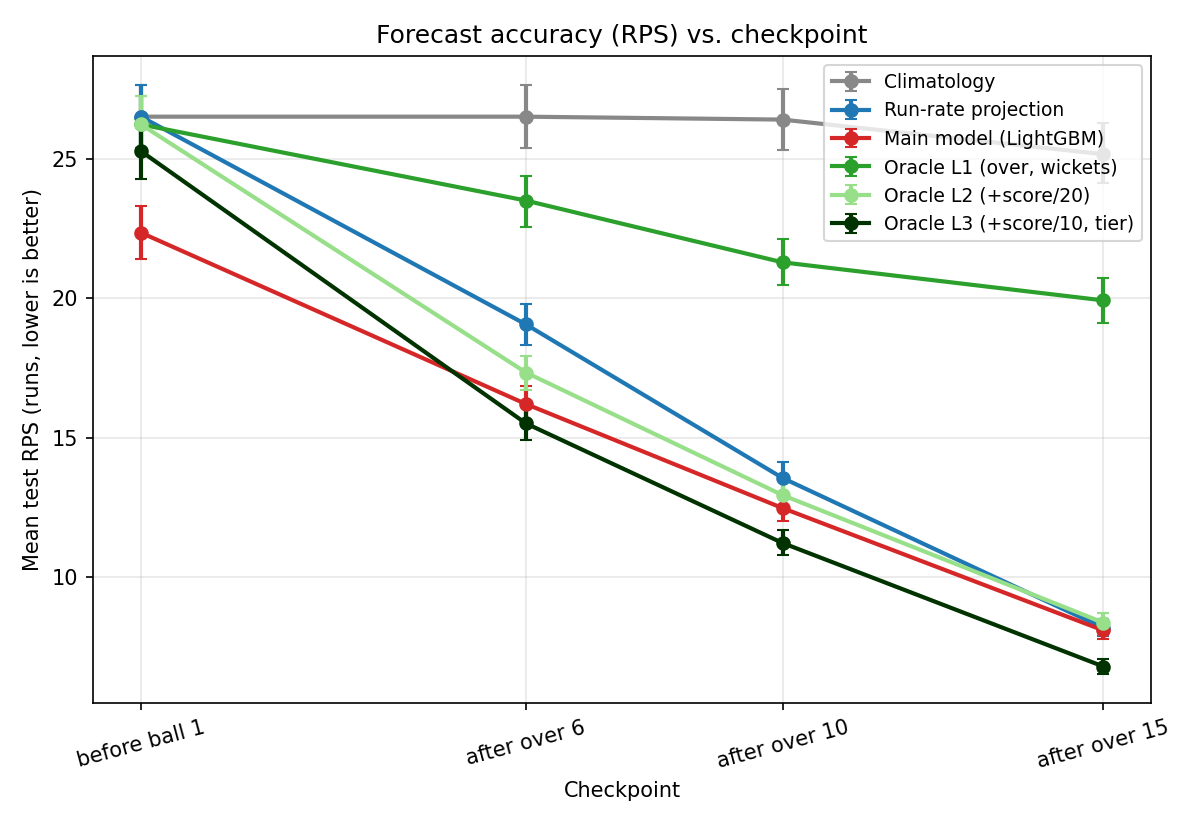
\includegraphics[width=0.7\linewidth]{figs/rps_vs_checkpoint.png}
\caption{Mean test RPS by checkpoint with 95\% bootstrap intervals.}
\label{fig:rps}
\end{figure}

\subsection{Q5.1: The optimal score given the features}\label{sec:oracle}
Let $X$ denote the information available at a checkpoint and $G(\cdot \mid X)$ the true conditional distribution of $Y$. By Eq.~\eqref{eq:decomp}, the best any forecaster using $X$ can do is to report $G(\cdot\mid X)$, which attains the \emph{Bayes risk}
\begin{equation}
R^*(X) = \E_X \Big[ \sum_{t} G(t\mid X)\big(1 - G(t\mid X)\big) \Big].
\end{equation}
This is the optimal score for the features at hand. Two facts guide how we estimate it.

\textbf{More information never hurts.} If $A$ is a function of $X$ (a coarsening), then $R^*(X) \le R^*(A)$: since $G(t\mid A) = \E[G(t\mid X)\mid A]$ and $x \mapsto x(1-x)$ is concave, Jensen's inequality gives $\E[G(t\mid X)(1-G(t\mid X))] \le \E[G(t\mid A)(1-G(t\mid A))]$ for each $t$.

\textbf{Estimating it with known outcomes.} Because we know the test outcomes, we can estimate $R^*(A)$ for a coarse $A$ directly: partition the test rows into bins by $A$, use the empirical distribution of $Y$ within each bin as the forecast, and score it on the same rows. We use three levels: L1 bins on (over, wickets); L2 adds the score in 20-run buckets; L3 uses 10-run buckets and adds the batting team's tier. This in-sample estimate is optimistic, by an amount we can compute exactly:

\begin{lemma}[In-sample bias]\label{lem:bias}
In a bin of $n$ i.i.d.\ outcomes with true CDF $G$, the in-sample RPS of the empirical CDF $\hat G$ equals $\sum_t \hat G(t)(1-\hat G(t))$, and its expectation is $\frac{n-1}{n}\sum_t G(t)(1-G(t))$.
\end{lemma}
\begin{proof}
With $Z_{it} = \1\{y_i \le t\}$ and $\hat G(t) = \frac1n\sum_i Z_{it}$, we get $\frac1n\sum_i (\hat G(t) - Z_{it})^2 = \hat G(t) - \hat G(t)^2$ because $Z_{it}^2 = Z_{it}$. Then $\E[\hat G(t)^2] = G(t)^2 + G(t)(1-G(t))/n$, so $\E[\hat G(t)(1-\hat G(t))] = (1 - \tfrac1n)\,G(t)(1-G(t))$.
\end{proof}

So a bin of size 1 always scores 0, and a bin of size 3 scores on average two thirds of its true Bayes risk. Table~\ref{tab:bins} shows why this matters: at over 15, L3 splits 1{,}439 rows into 202 bins with a median size of 3, so its score of 6.78 is substantially optimistic. L1 has large bins and a negligible bias, but it conditions on so little that its Bayes risk is far above that of the richer feature set. An unbiased estimate of each level's Bayes risk rescales every bin with $n \ge 2$ by $n/(n-1)$. The true optimum for the model's features, $R^*(X)$, lies below the population value of $R^*(\text{L2})$, since L2's bins are functions of the model's inputs.

\begin{table}[!htbp]
\centering
\caption{Oracle binning: number of bins and median bin size on the test set.}
\label{tab:bins}
\small
\begin{tabular}{lrrrrrr}
\toprule
 & \multicolumn{2}{c}{L1: over, wickets} & \multicolumn{2}{c}{L2: + score/20} & \multicolumn{2}{c}{L3: + score/10, tier} \\
\cmidrule(lr){2-3}\cmidrule(lr){4-5}\cmidrule(lr){6-7}
Checkpoint & Bins & Median size & Bins & Median size & Bins & Median size \\
\midrule
Before ball 1 & 1  & 1{,}479 & 1  & 1{,}479 & 2   & 739.5 \\
After over 6  & 8  & 172.5   & 30 & 16.5    & 87  & 6 \\
After over 10 & 11 & 68      & 55 & 10      & 143 & 5 \\
After over 15 & 11 & 115     & 79 & 8       & 202 & 3 \\
\bottomrule
\end{tabular}
\end{table}

\section{Results (Q5.2)}\label{sec:results}


Table~\ref{tab:main} and Figure~\ref{fig:rps} summarize the results.

\textbf{The model is most valuable early.} Before ball 1, neither baseline can distinguish between matches, while the model uses the teams, players and venue to reduce RPS from 26.52 to 22.35 runs (skill 0.16). Its advantage over the run-rate projection then shrinks from 4.16 runs to 2.86, 1.08 and 0.09 runs at overs 6, 10 and 15. By over 15, score, wickets and overs remaining explain most of what can be known, and the intervals of the model and the projection overlap almost entirely. Skill relative to climatology rises over the innings (0.16 to 0.68) only because climatology ignores the innings state.

\textbf{Distribution shift is small at the marginal level.} Before ball 1, L1 and L2 are a single bin, i.e.\ the empirical distribution of test totals. It scores 26.24 against climatology's 26.52: knowing the test-period marginal distribution in advance would gain only 0.28 runs.

\textbf{Comparison with the optimal score.} The model beats oracles L1 and L2 at every checkpoint, by 0.28--1.13 runs against L2 after the first ball. This does not contradict their role as optimal scores: they are optimal only for their coarse features, and the model sees much more. L3 conditions more finely and beats the model by 0.70, 1.25 and 1.30 runs at overs 6, 10 and 15. By Lemma~\ref{lem:bias}, much of this gap comes from L3's small bins rather than exploitable signal. We therefore read the gap to L3 as an upper bound on the achievable improvement, and the model's lead over L2 as evidence that it is extracting information beyond the coarse state.

\begin{figure}[!htbp]
\centering
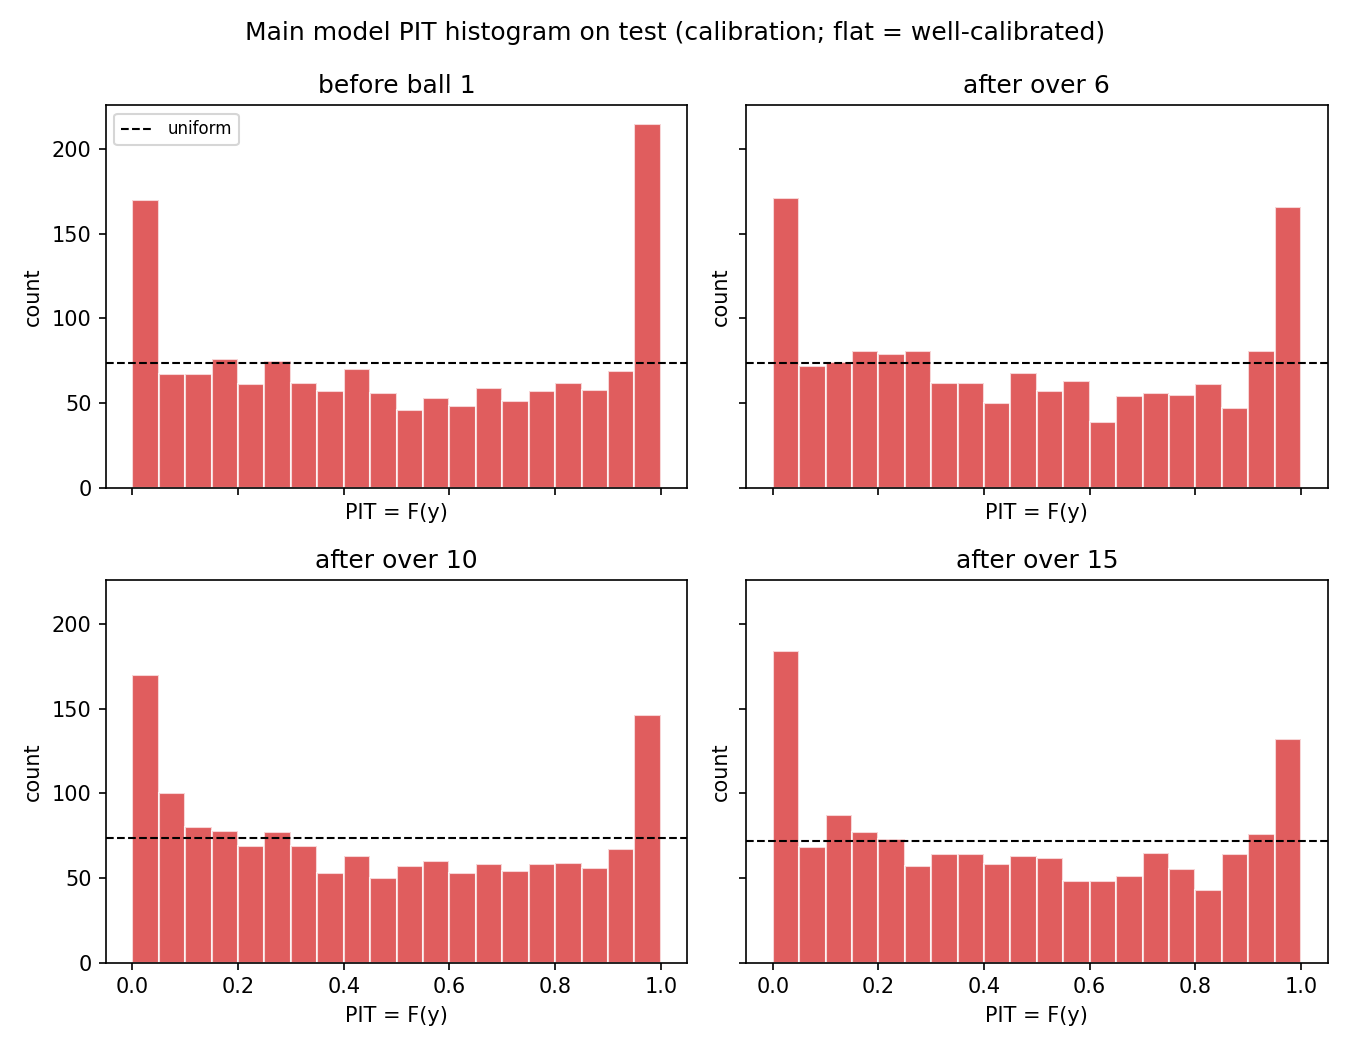
\includegraphics[width=0.86\linewidth]{figs/pit_histogram.png}
\caption{Probability integral transform $F(y)$ of the main model on test. A calibrated forecaster gives a flat histogram (dashed line). The U shape indicates overconfidence.}
\label{fig:pit}
\end{figure}

\textbf{Calibration.} Figure~\ref{fig:pit} shows PIT histograms~\citep{dawid1984}. All four are U-shaped. The outer bins, $F(y) < 0.05$ and $F(y) > 0.95$, should each hold 5\% of outcomes; reading from the histograms, together they hold about 22--26\%. The model's nominal 90\% intervals therefore cover only about 74--79\% of test totals. This is not caused by anchoring the CDF at 0 and 300: whether $y$ falls below the 0.05 quantile does not depend on how the tail beyond that quantile is drawn. The quantile models themselves are too narrow on test data. Before ball 1, the right bin is the tallest, meaning high totals are underpredicted, which is consistent with scoring rates in 2024 and later exceeding those in the training period. After over 15, the left bin dominates, meaning late collapses are underpredicted. Because RPS is proper, correcting these errors should also lower the score.

\begin{figure}[!htbp]
\centering
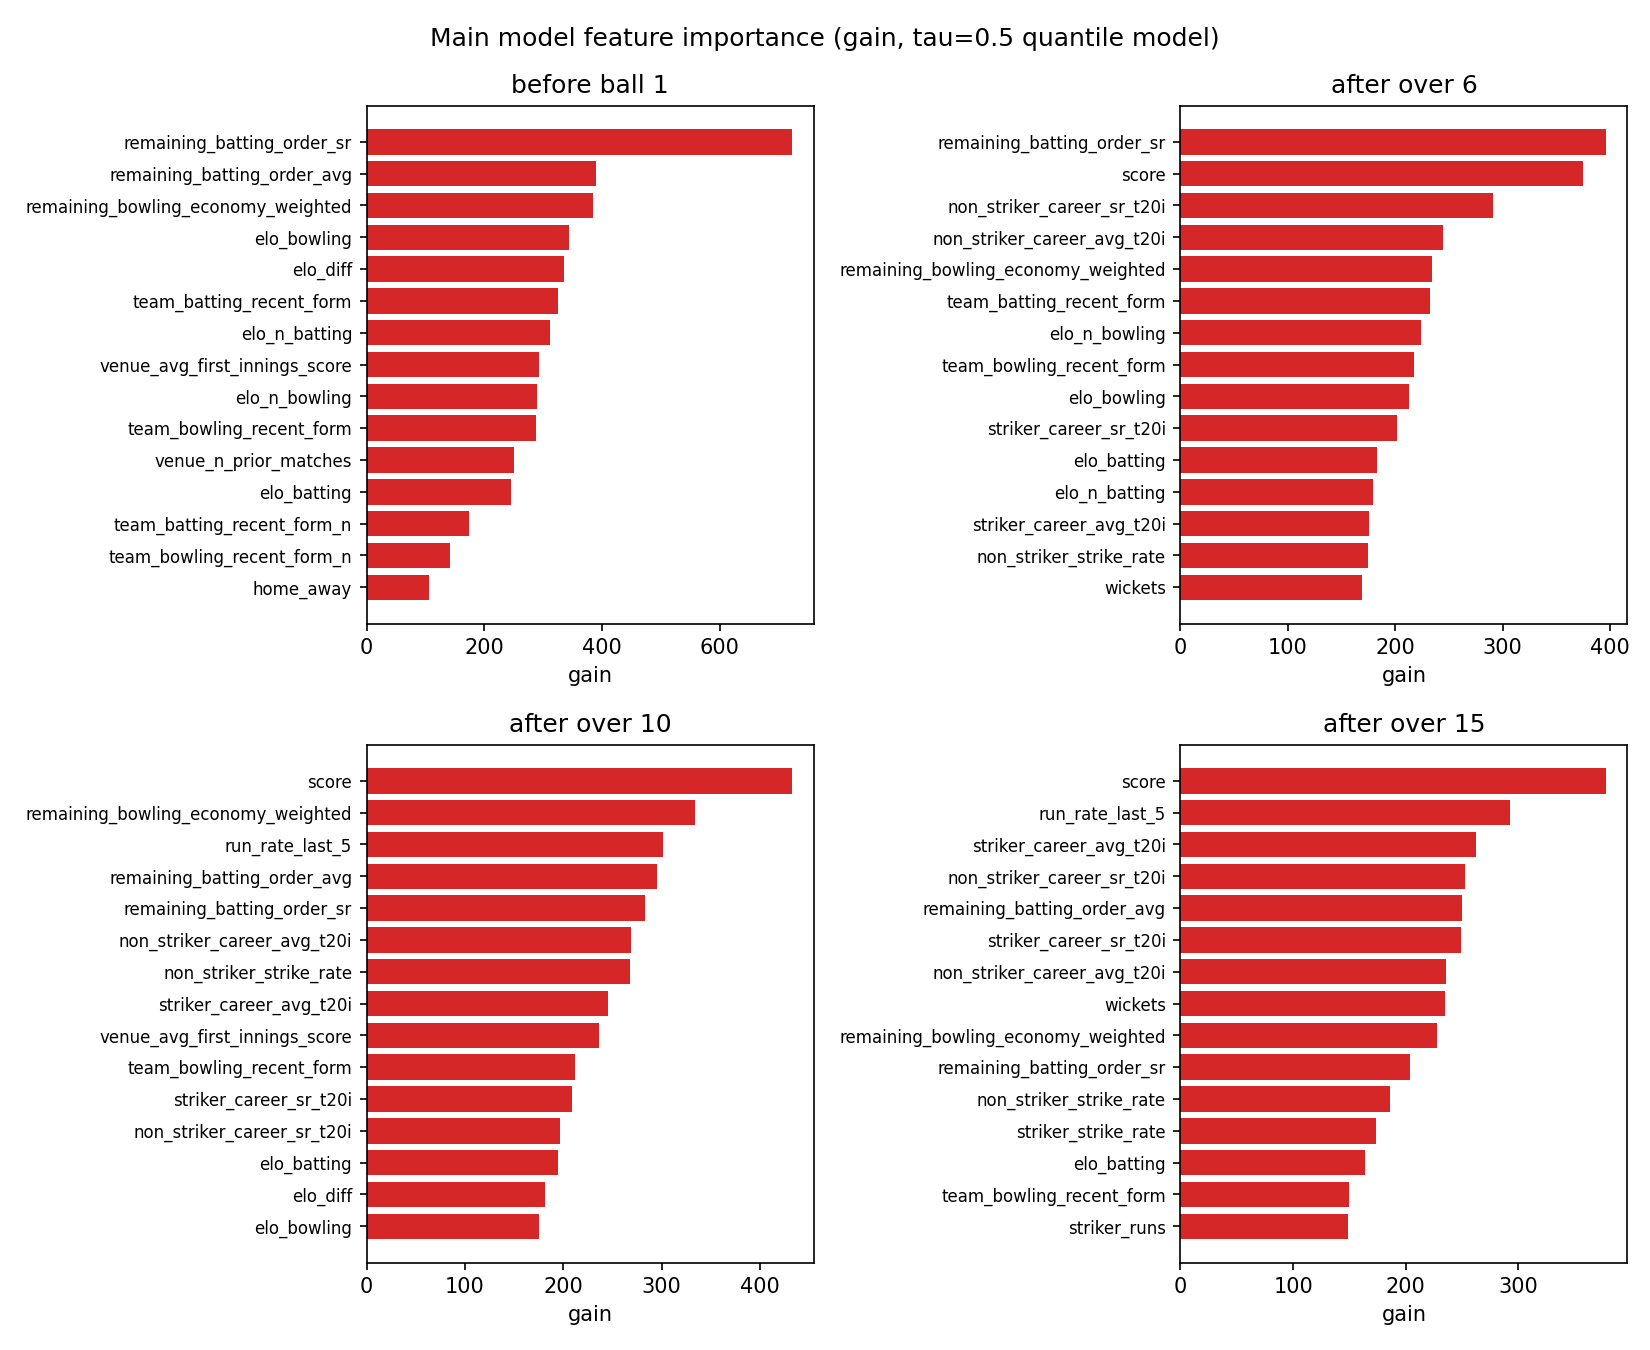
\includegraphics[width=\linewidth]{figs/feature_importance.png}
\caption{Top 15 features by gain for the median ($\tau = 0.5$) quantile model at each checkpoint.}
\label{fig:importance}
\end{figure}

\textbf{What the model uses.} Figure~\ref{fig:importance} shows that before ball 1 the strength of the batting order (career strike rate and average of the XI) dominates, followed by the bowling side's economy, Elo ratings, recent form and venue average. As the innings progresses, the current score rises to the top, and by over 15 the most useful signals are the score, the run rate over the last five overs and the quality of the two batters at the crease. This matches the intuition that pre-match context matters early and the innings state matters late.

\subsection{Is the method improvable?}\label{sec:improve}
Yes, especially early in the innings, where the gap to the fine-grained oracle is largest in relative terms and the model's advantage over simple baselines comes from context features. We expect the following changes to help, in rough order of expected benefit:
\begin{enumerate}
\item \textbf{Recalibration.} Widen the predictive distributions using the validation year, for instance with conformalized quantile regression~\citep{romano2019} or a spread factor chosen to minimize validation RPS. The PIT histograms show a clear, fixable miscalibration.
\item \textbf{Use all the data and adapt to drift.} The model is fit on data up to 2022 only; refitting on training plus validation data, and weighting recent seasons more heavily, should reduce the underprediction of high totals.
\item \textbf{Richer player histories.} Many associate players have few T20Is. Ratings computed from all men's T20 cricket on Cricsheet, including franchise leagues, would be less noisy.
\item \textbf{A wider tuning grid and a pooled model.} The selected configuration was the smallest in the grid, so more regularized models may do better. A single model across all balls, with balls remaining as a feature, would share strength across checkpoints.
\item \textbf{Information outside Cricsheet.} Weather, dew, day/night scheduling and pitch reports are unavailable to us and plausibly matter, especially before ball 1.
\end{enumerate}
Improvement is limited late in the innings. After over 15 the model is statistically indistinguishable from the run-rate projection, and even the optimistic L3 oracle scores 6.78 runs: most of the remaining uncertainty is the irreducible randomness of the final five overs.

\section{Conclusion}
Ball-by-ball Cricsheet data support honest backtesting of in-play forecasts of T20I first-innings totals. The Ranked Probability Score, derived as a sum of threshold Brier scores, is strictly proper and measured in runs. A LightGBM quantile model beats climatology and run-rate baselines, particularly before the innings starts, and beats coarse-feature oracles. The remaining gap to a fine-grained oracle is partly an artifact of in-sample estimation, which we quantified exactly, and the clearest fixable weakness is overconfidence.

\small
\begin{thebibliography}{99}

\bibitem{brier1950}
G.~W. Brier.
\newblock Verification of forecasts expressed in terms of probability.
\newblock \emph{Monthly Weather Review}, 78(1):1--3, 1950.

\bibitem{cricsheet}
Cricsheet.
\newblock Freely-available structured data for cricket.
\newblock \url{https://cricsheet.org}.

\bibitem{dawid1984}
A.~P. Dawid.
\newblock Present position and potential developments: Some personal views. Statistical theory: The prequential approach.
\newblock \emph{Journal of the Royal Statistical Society, Series A}, 147(2):278--292, 1984.

\bibitem{elo1978}
A.~E. Elo.
\newblock \emph{The Rating of Chessplayers, Past and Present}.
\newblock Arco, 1978.

\bibitem{epstein1969}
E.~S. Epstein.
\newblock A scoring system for probability forecasts of ranked categories.
\newblock \emph{Journal of Applied Meteorology}, 8(6):985--987, 1969.

\bibitem{gneiting2007}
T.~Gneiting and A.~E. Raftery.
\newblock Strictly proper scoring rules, prediction, and estimation.
\newblock \emph{Journal of the American Statistical Association}, 102(477):359--378, 2007.

\bibitem{ke2017}
G.~Ke, Q.~Meng, T.~Finley, T.~Wang, W.~Chen, W.~Ma, Q.~Ye, and T.-Y. Liu.
\newblock {LightGBM}: A highly efficient gradient boosting decision tree.
\newblock In \emph{Advances in Neural Information Processing Systems}, 2017.

\bibitem{koenker1978}
R.~Koenker and G.~Bassett.
\newblock Regression quantiles.
\newblock \emph{Econometrica}, 46(1):33--50, 1978.

\bibitem{matheson1976}
J.~E. Matheson and R.~L. Winkler.
\newblock Scoring rules for continuous probability distributions.
\newblock \emph{Management Science}, 22(10):1087--1096, 1976.

\bibitem{romano2019}
Y.~Romano, E.~Patterson, and E.~Cand\`es.
\newblock Conformalized quantile regression.
\newblock In \emph{Advances in Neural Information Processing Systems}, 2019.

\end{thebibliography}

\end{document}
